\documentclass{beamer}
\usetheme{Madrid}

\usepackage{amsmath, amssymb, amsthm}
\usepackage{graphicx}
\usepackage{gensymb}
\usepackage[utf8]{inputenc}
\usepackage{hyperref}
\usepackage{tikz}
\usepackage{amsmath}

\title{5.3.6 Matgeo}
\author{AI25BTECH11012 - Garige Unnathi}
\date{}

\begin{document}

\frame{\titlepage}

% Question frame
\begin{frame}
\frametitle{Question}
If the pair of equations 3x - y + 8 = 0 and 6x - ry + 16 = 0 represents coincident
lines, then the value of r is 
\end{frame}


% Solution steps
\begin{frame}
\frametitle{Solution}
Let :
\begin{align}
\mathbf{r_1} = \begin{bmatrix}3 & -1\end{bmatrix}\mathbf{x} = -8 \\
\mathbf{r_2} = \begin{bmatrix}6 & -r\end{bmatrix}\mathbf{x} = -16
\end{align}
For coincident lines:
\begin{align}
   Rank( \textbf{$r_1$} \quad \textbf{$r_2$})  = \begin{bmatrix}3 & -1\\
                                              6 & -r\end{bmatrix} = 1
\end{align}

solving using above equation :
\begin{align}
   R_2 = R_2 - 2R_1\\
   =  \begin{bmatrix}3 & -1\\
                      0 & -r + 2\end{bmatrix} = 1
\end{align}
\end{frame}



\begin{frame}
\frametitle{Solution}
For the rank of above matrix to be one ,we need :

\begin{align}
   -r + 2 =0 \\
   r = 2 
\end{align}
\end{frame}


\begin{frame}
\frametitle{Graphical Representation}

\begin{center}
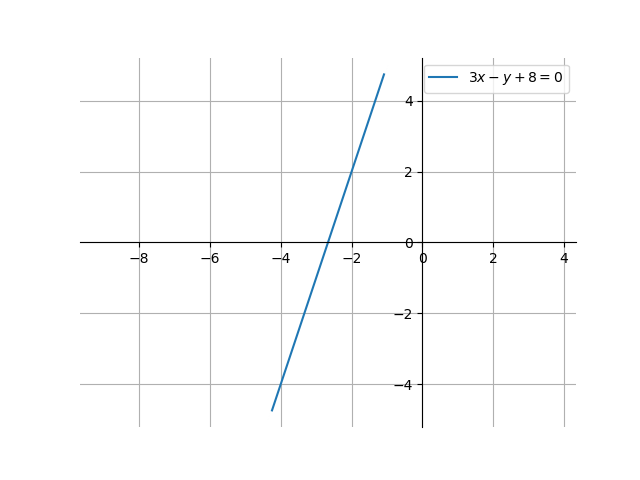
\includegraphics[width=0.6\linewidth]{/Users/unnathi/Documents/ee1030-2025/ai25btech11012/matgeo/5.3.6/figs/figs.png}
\end{center}
\end{frame}

\end{document}
